%!TEX program = xelatex
\documentclass[12pt, a4paper, oneside]{ctexart}
\usepackage[utf8]{inputenc}
\usepackage{ctex} %导入中文包
\usepackage{listings}
\usepackage{fontspec}
\usepackage{geometry} %设置页边距的包
\usepackage{listings}
\usepackage{xcolor} 
\usepackage{graphicx}
\usepackage{float}


\title{\fontsize{70}{30}\selectfont  ACM 算法模板} 
\author{Buns\_out} 
\date{\today} 

\geometry{left=2.5cm,right=2cm,top=2.54cm,bottom=2.54cm} %设置书籍的页边距
\definecolor{mygray}{rgb}{0.97,0.97,0.97}%定制颜色

\setsansfont{Monaco} 
\setmainfont{Monaco}


%对于lstset排版
\lstset{
tabsize=4,
	breaklines, 					% 自动将长的代码行换行排版
	backgroundcolor = \color{white},     			 % 背景色:淡黄
	numbers=left, 									% 行号在左侧显示
	numberstyle= \small, 								% 行号字体
	keywordstyle= \color{ red!70},						 % 关键字颜色
	commentstyle= \color{red!50!green!50!blue!50}, 		% 注释颜色
	rulesepcolor= \color{ red!20!green!20!blue!20} ,
	frame=single,                               % 设置代码框形式
	escapeinside=``,									 % 英文分号中可写入中文
	xleftmargin=2em,xrightmargin=2em, aboveskip=1em,
	framexleftmargin=2em
} 


\begin{document} 


% \maketitle
% \thispagestyle{empty}
% \centering
% 
\includegraphics[scale=1.0]{pic.png}

\newpage
\section{ 网络流建图 } 
\subsection{ 最小路径覆盖 } 
\textbf{最小路径覆盖 }: \par
\qquad 在一个有向无环图中,找出最少的路径,使得这些路径经过了所有的点。最小路径覆盖分为\textbf{最小不相交路径覆盖}和\textbf{最小可相交路径覆盖},区别是这些路径是否可以相交

\subsubsection{ 最小不相交路径覆盖 }
建图方法:\par
\qquad 把原图的每个点u拆成两个点$u_{1}$,$u_{2}$,如果有一条有向边$(a,b)$,则连边$(a_{2},b_{1})$,容易发现这是一个二分图,那么用下面的定理就可以求出答案
\par
定理: 最小路径覆盖=原图节点数-新图最大匹配数
\par
证明:
\par
\qquad 一开始每个点都是一条路径,每次找一条匹配边,代表合并两条路径\\
由于路径不相交(即每个点的入度和出度至少有一个为$1$),所以二分图上的边也不相交(如果相交则说明某个点的入度或出度大于$1$),这正好是匹配的定义\\
每条匹配边代表答案$-1$,所以\textbf{最小路径覆盖=原图节点数-新图最大匹配数}

\subsubsection{最小可相交路径覆盖}
\qquad 对原图传递闭包,即若原图中$(u,v)$连通,则增加边$(u,v)$.这可以用$Floyd$算法$O(n^{3})$实现。然后对新图做最小不相交路径覆盖即可。因为在原图中相交的路径在传递闭包后可以拆分成另一条边,这样就不相交了

\subsubsection{最多不相交路径} 
\qquad  这种问题变化比较多,但都能表示成以下形式:
\par 
\textbf{已知一些路径,每个节点只能属于一条路径,求能选择多少条路径使它们不相交.}
\par
\qquad  主要的方法是拆点,将一个点拆成两个,然后连边,容量表示该点最多经过次数

\newpage
\subsection{最小割}
\subsubsection{最大权闭合子图}
\textbf{定义:}
\par
\qquad  有一个有向图,每一个点都有一个权值,选择一个权值和最大的子图,使得每个点的后继都在子图里面,这个子图就叫最大权闭合子图。\par
\textbf{建图方法:}
\par
\qquad  从源点s向每个正权点连一条容量为权值的边,每个负权点向汇点t连一条容量为权值的绝对值的边,有向图原来的边容量全部为无限大。\par
\textbf{定理}:
\par
\qquad  最大权闭合子图=所有正权点之和-最小割\par
\textbf{关键性质}:
\par
\qquad  如果$s$与$i$有边,表示$i$在子图中。如果$i$与$t$有边,表示$i$不在于子图中。即:割掉$s$与$i$表示不选$i$,割掉$i$与$t$表示选$i$。\par
\textbf{性质$1$}:
\par
\qquad  原图之间的边一定不会被割掉\par
 边权为无穷大,当然不会被选进最小割\par
\textbf{性质$2$}:
\par
\qquad  只有$s$到$t$不联通时,才得到最大权闭合子图\par
\textbf{反证法}:
\par
\qquad  若$s$到$t$连通,则一定存在节点$i$,$j$使$s$到$i$有边,$i$到j有边(引理$1$),$j$到$t$有边.而根据性质$1$:$i$在子图中,$j$不在子图中,这与最大权闭合子图的定义矛盾,证毕
由引理$2$可得,图的一个割就是一个闭合子图\par
由于一个割的边权和=不选的正权点+选的负权点绝对值=不选的正权点−选的负权点一个割的边权和=不选的正权点+选的负权点绝对值=不选的正权点−选的负权点.\par
闭合子图=正权点+负权点=所有正权和−不选的正权点+选的负权点=所有正权和−割的边权和闭合子图=正权点+负权点=所有正权和−不选的正权点+选的负权点=所有正权和−割的边权和\par
显然割的边权和最小的时候得到最大权闭合子图,证毕

\newpage
\subsection{最小割}
\textbf{定理:} \par
\qquad  二分图最大独立集=$n$-二分图最大匹配\par
\qquad  其实二分图独立集是\textbf{特殊的一种最大权闭合子图}。我们根据上文“收益”的思想,把选某个点的收益看为$1$,左部节点为正权点,右部节点为负权点.按照最大权闭合子图的方式建图,答案为正权和-最小割=$n$-最小割=$n$-最大流。我们发现把最大权闭合子图中$INF$的边换成$1$也不影响答案,因为图中其他边的容量都为$1$。这样图就变成了二分图匹配中的图,最大流=二分图最大匹配


\subsection{最大密度子图}
\textbf{定义}:图的密度是图上的边的数量除以点数。求密度最大的子图。\par
\textbf{建图}:看到平均数想到01分数规划。二分答案$mid$,那么问题转化为判定是否存在一个子图,使得边数−$mid\cdot$点数$>$ $0$边数−$mid \cdot$点数>$0$.那么可以把每条边的权看成$1$,每个点的权看成$−mid$,限制是选择一条边就必须选择边连接的两个点。于是把边看成左部点,点看成右部点,跑最大权闭合子图,若答案$>0$,则合法。


\subsection{二元关系最小割模型}
\textbf{定义}:有若干个变量,每个变量有2种取值,有若干个现在,每个限制形如"若变量$x=a,y=b$,就要付出$c$的代价"。最大化所有变量的值之和减去最小代价。\par
\textbf{建图}:每个变量建一个点,$S$到$x$连边表示$x$的一种取值的代价,$x$到$T$连边表示$x$的另一种取值的代价。对于一个限制,在两个点之间连边。边权需要列方程解出。


\subsection{二分图带权匹配}
\textbf{定义}:每条边有边权,求匹配边权值之和最大的匹配\par
\textbf{建图}:在边上加上权,跑费用流即可


\subsection{最大权不相交路径}
\textbf{定义}:每条路径有一个权值(一般是边权和),在**不相交路径数最多的情况下**,最大化费用\par
\textbf{建图}:同最多不相交路径,在连接两个拆点的边上加上费用跑费用流即可


\subsection{不等式差分模型(网络流解线性规划)}
\textbf{定义}:对于一些不太好直接想到建图的问题,我们可以数学建模,列出方程然后用线性规划求解。这样的好处是思维量较小,只要做代数变换就可以建图,而不用考虑建图的实际意义。我们需要把式子做差,使得每个未知数仅在两个等式中出现。\par
根据网络流中每个点流量平衡的思想,我们可以把$−xi$看成从点$i$流出$x_{i}$的流量,$+x_{i}$看成流入$x_{i}$的流量。等式为$0$就代表流量平衡。\par
\textbf{建图}:每个等式为图中一个顶点,添加源点$S$和汇点$T$。\\
如果一个等式右边为非负整数$c$,从源点S向该等式对应的顶点连接一条容量为$c$,权值为$0$的有向边;如果一个等式右边为负整数$c$,从该等式对应的顶点向汇点$T$连接一条容量为$c$,权值为$0$的有向边。\\
如果一个变量$x_{i}$在第$j$个等式中出现为$x_{i}$,在第$k$个等式中出现为$-x_{i}$,且在目标函数里的系数为$c_{i}$,从顶点j向顶点k连接一条容量为$+\infty$,费用为$c_{i}$的有向边。\\
- 如果一个变量$y_{i}$在第$j$个等式中出现为$y_{i}$,在第$k$个等式中出现为$-y_{i}$,且在目标函数里没有出现,从顶点j向顶点k连接一条容量为$+\infty$,权值为$0$的有向边。


\subsection{有上下界的网络流}
\subsubsection{无源汇有上下界可行流}

\textbf{定义:}无源汇网络指的是\textbf{没有源点和汇点},每个点都有入边和出边且满足流量守恒即满足上下界要求的网络。在这个网络上求一个流量方案,使得每条边的流量必须在$[l_{i},r_{i}]$之间,且每个点流量守恒。\par

有上下界的费用流的核心是\textbf{补偿}。我们先假设每条边的流量均为 $l_{i}$,那么一定会有一些点流量不守恒。现在我们需要构造一个附加网络,使得把附加网络和原网络叠加(即对应边流量相加)之后的图满足流量守恒。\par

如下图,将原网络拆分为两个结构与原图相同的普通网络,左图边界的容量为原网络对应边界的 $l_{i}$ 下界,另一个为对应边的上下界流量之差,即 $l_{i} - r_{i}$ 。

\centering % 中间对齐
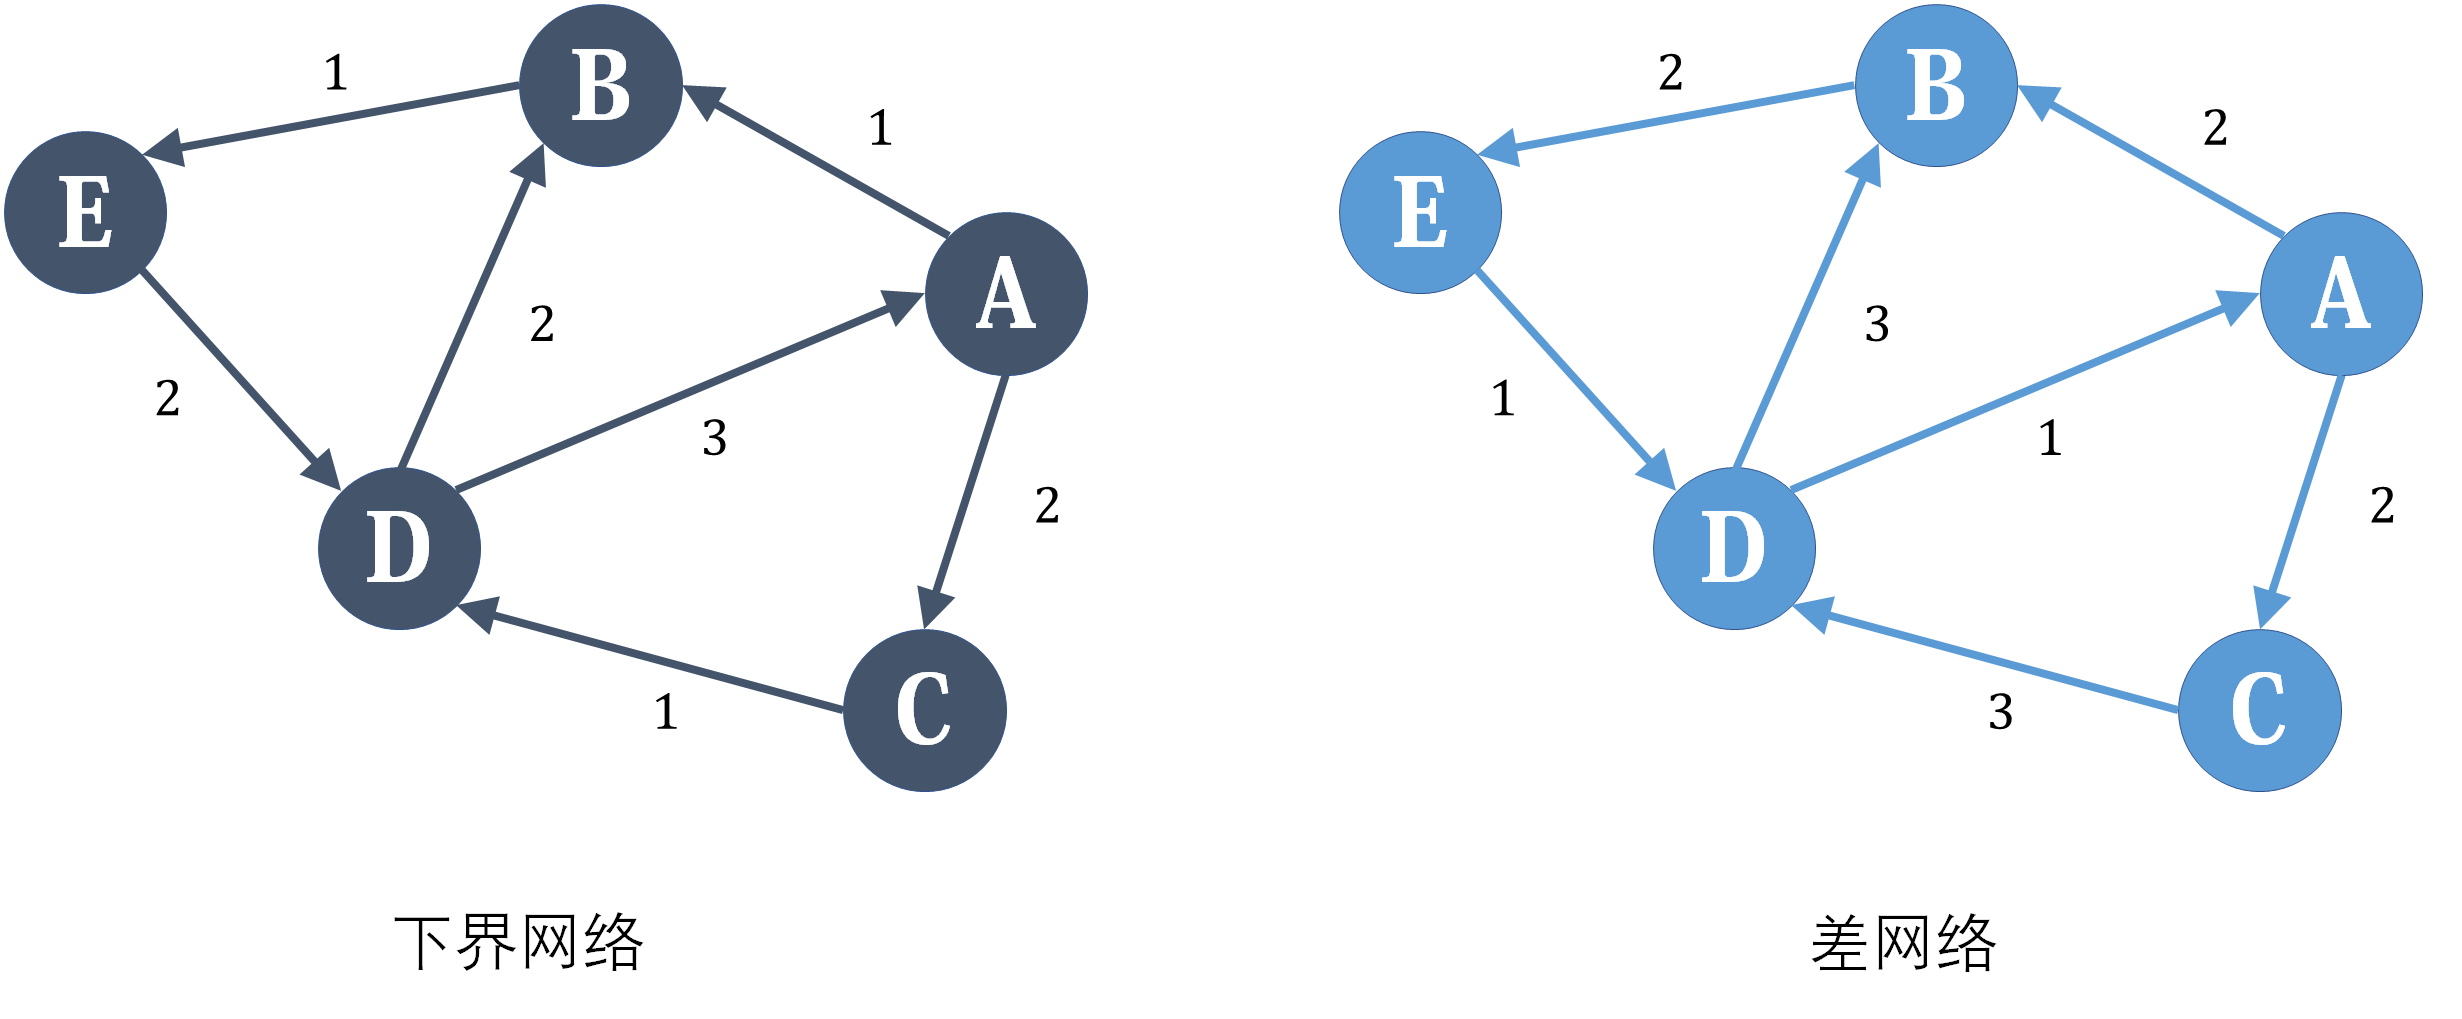
\includegraphics[scale=0.18]{pic1.png}
\flushleft % 左对齐

\qquad 我们希望下届网络和差网络相加后恰好是原图的一个可行流,这首先要求下届网络是满流的(可行流必须达到每条边的下界)。但是下界网络满流之后不一定流量平衡,所以我们要对差网络进行一定的修改弥补这种不平衡。\par
	
\qquad 我们分别考虑下界网络的每个点。$A$ 点,流入量为$3$,流出量也为 $3$,$A$ 点平衡。那么在差网络中也是平衡的,所以不做修改。$B$ 点,流入量为 $3$,流出量为 $1$,流入比流出多 $2$,那么我们希望在差网络中,$B$ 的流出应该比流入多 $2$,于是我们在差网络中新设立一个\textbf{源点},然后加入一条流量为 $2$ 的\textbf{附加边}从源点到 $B$ 点,这样在差网络平衡是,出去附加边,$B$ 点的流出恰好比流入多 $2$。$C$ 点与 $B$ 点类似,然而 $D$ 点相反。我们希望在差网络中 $D$ 点流入比流出多 $2$,所以新设立一个\textbf{汇点},然后从 $D$ 点连一条容量为 $2$ 的附加边到汇点,$E$ 点与 $D$ 点类似。\par

\qquad 也就是说,如果下界网络中某个点有 $x$ 的净流入,在差网络中我们就从源点向它连一条容量为 $x$ 的附加边;相反,如果下界网络中某个点有 $x$ 的净流出,在差网络中我们就从它向汇点连一条容量为 $x$ 的附加边。这样,我们把差网络修改如下:\par

\centering % 中间对齐
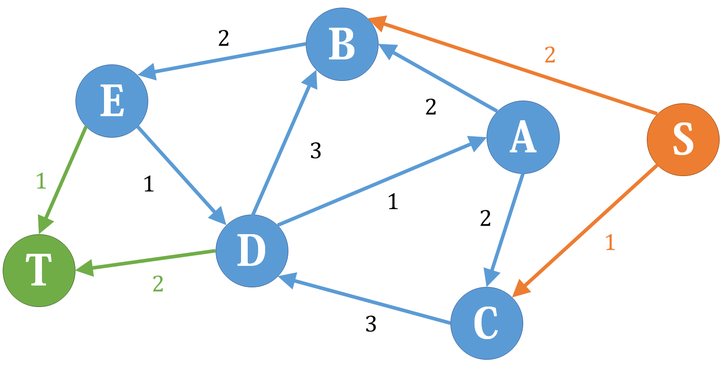
\includegraphics[scale=0.4]{pic2.png}
\flushleft % 左对齐


\qquad 在差网络上跑一遍最大流,把每条非附加边的流,加上下界网络的满流,就是一个可行流。但是,如果跑完最大流发现,存在\textbf{附加边未满流},那说明平衡条件没有得到满足,于是原图不存在可行流。\par

\qquad 在实际中,是不需要建立下界网络的,只需要对差网络进行操作即可。另外最后判断的时候\textbf{并无必要遍历所有附加边},而只需要判断所有从源点出发的边,或者判断所有连向汇点的边即可,因为根据网络流的性质,两者容量和应该相等,于是它们要么都满流,要么都不满流。\par

\qquad 因为 $DINIC$ 只能求有源汇最大流,所以是不能直接求出附加网络的流量的。那么我们可以在附加网络上添加一些不在原网络上的边和点,来实现我们的限制.\par
记 $d_{i}=$ 点 $D$ 的入流 $-$ 点 $i$ 的出流,然后建附加网络:\par
1.新建源点$ss$和汇点$tt$\par
2.对于原图中的每条边$e_{i}=(u,v)$,连边$(u,v,r_{i}-l_{i})$,也就是说附加网络包括原网络的边。\par
3.新建边来满足流量守恒\par
若$d_{i}=0$则该点流量平衡,不用处理\par
若$d_{i}>0$则入流D$>$出流,那么附加网络中$i$的出边需要增加流量,我们连边$(ss,i,d_{i})$,这样求最大流的时候出边的流量会增加$d+{i}$,叠加后满足流量守恒\par
若$d_[i]<0$则入流$<$出流,那么附加网络中$i$的入边需要增加流量,同理连边$(i,tt,-d_{i})$,这样求最大流的时候入边的流量会增加$-d_{i}$,叠加后满足流量守恒\\
那么当且仅当步骤3中新建边满流时有解,总可行流为$maxfolw(ss,tt)+\sum{l_{i}}$。每条边在原图中流量=容量下界+附加流中它的流量

\subsubsection{有源汇有上下界可行流}
\textbf{定义}:在有源汇网络上求一个流量方案,使得每条边的流量必须在$[l_{i},r_{i}]$之间,且除源汇外每个点流量守恒。\par
设原网络的源和汇分别为$s,t$我们在原网络上加一条边${(t,s,+\infty)}$,相当于把到汇点的所有流量都流回源点,这样每个点流量都守恒。\par
\qquad 然后套无源汇的方法即可。因为此时的源点汇点已经被处理成普通点。\par
\qquad 注意 此时总流量 $=$  $t$ 到 $s$ 的无穷边在原图中的流量。

\centering % 中间对齐
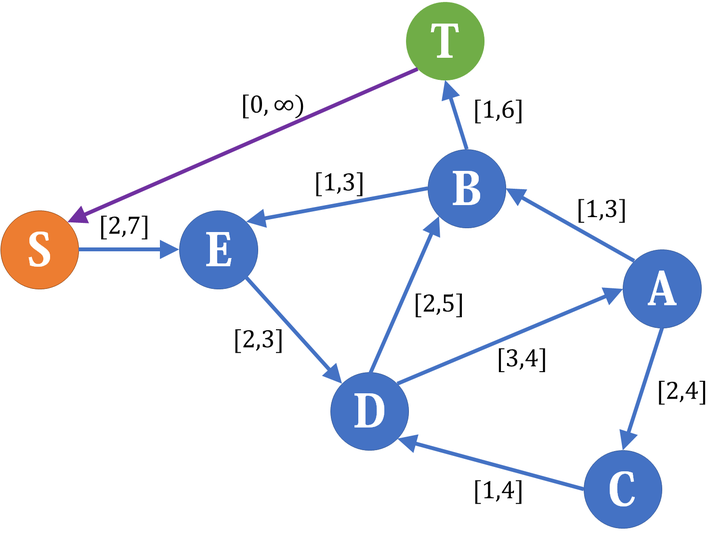
\includegraphics[scale=0.4]{pic3.png}
\flushleft % 左对齐


\subsubsection{有源汇有上下界最大流和最小流}
\textbf{定义}:在有源汇网络上求一个流量方案,使得每条边的流量必须在$[l_{i},r_{i}]$之间,且除源汇外每个点流量守恒。在这个条件下使得总流量最大/最小。\par
先按上面的方法求出一个有源汇有上下界可行流.然后在附加网络上再跑一次$s$到$t$的最大流(注意不是$ss$,$tt$!)。最大流=可行流+第二次跑的$s$到$t$最大流。\par
再跑一次最大流是因为附加网络上属于原图的边还有流量没被“榨干”。容易发现只要附加网络上不属于原图的边满流,属于原图的边怎么跑流量都是守恒的。因为第一次跑最大流已经保证所有点守恒,第二次跑最大流不会经过不属于原图的边,因此等价于对原图跑一次普通的最大流,除源汇外流量守恒。两次合起来总流量一定守恒,这就保证了正确性。\par
同理求最小流就跑一次$t$到$s$的最大流。最小流=可行流-第二次跑的t到s最大流。这是因为Dinic过程中反向边的流量增加等价于正向边的的流量减少。

\subsubsection{有源汇有上下界最小费用流}
\textbf{定义}:在有源汇网络上求一个流量方案,使得每条边的流量必须在$[l_{i},r_{i}]$之间,且除源汇外每个点流量守恒。每条边单位流量的费用为$c_{i}$.在这个条件下使得总费用最小,费用定义同一般费用流。(不要求总流量最大)\par
这是有上下界费用流常被误解的一点,即最小费用流求的是费用最小的可行流,而不是最大流。\\

因此按有源汇可行流的方法建图,把原图中的边带上费用。总费用$=mincost(ss,tt)+\sum{l_{i}c_{i}}$

\end{document}

